\chapter{\label{res3}Statistical modelling of evoked neural activity
}

\minitoc

To understand how neural activity is propagated between brain regions in order to guide behaviour, we used the all-optical methodology outlined in the previous two sections to compare the neural response during reported and non-reported stimuli (hit and miss trials respectively), both in the directly stimulated region (S1) and an anatomically connected downstream region (S2). 

\section{The structure of evoked activity in S1 and S2}

Qualitatively, hit trials elicit a diverse array of excitatory and inhibitory responses both in S1 and S2, whereas both excitatory and inhibitory responses were less obvious on miss trials. Excited and inhibited cells are also observed in ‘reward only’ trials (methods) in which reward was delivered in the absence of photostimulation, however the population response is less pronounced compared to hit trials, indicating that the response to reported stimulation is not just explained by neural activity driven by reward (Fig. 2a; Supplementary Fig. 2,3). We find that hit trials elicit a significantly greater fraction of responsive cells in S1 compared to all other trial types, whereas in S2, hit trials elicited a significantly greater fraction of responsive cells only compared to correct rejection and reward only trials (p < 0.05, Bonferroni corrected). The fraction of responsive cells was greater in S2 compared to miss and false positive trials but this result was not significant (p > 0.05, Bonferroni corrected) (Supplementary Fig. 1,a). On a single cell level, we find individual neurons in S2 that are excited or inhibited in response to hit trials, but not miss or reward only, hinting that reported stimuli are propagated to single neurons in S2 (Fig. 2b).

Interestingly however, averaging responses across cells, trials and sessions reveals that hit trials elicit only a modest increase in population activity from baseline, immediately following stimulation, in S1 and S2, followed by a prolonged period of inhibition. Whereas the reward only condition exhibited a very different time course (Fig. 2c,  Supplementary Fig. 1b,c). This hints that both brain regions exist in balanced regimes whereby excitation driven by photostimulation results in inhibition of roughly equal magnitude. Miss trials elicit excitation following photostimulation in S1, however this excitation is not observed as propagated activity in trial-and-cell-averaged responses downstream in S2 (Fig. 2c). 

We next compared how the percentage of excited or inhibited neurons, both locally in S1 and downstream in S2, scaled with the number of cells photostimulated in S1 and whether this differed between perceived and non-perceived stimuli (Fig. 2d,e). As expected, stimulating more neurons in S1 excited a greater percentage of the population regardless of whether the stimulus was perceived (Fig. 2d left) (Pearson’s r = 0.62, p  = 1.8x10-8 hit trials; Pearson’s r = 0.65, p = 2.4x10-9 miss trials). We also find that the percentage of inhibited cells in S1 also scales linearly with the number of cells stimulated (Fig. 2d right) (Pearson’s r = 0.55, p = 1.2x10-6 hit trials; Pearson’s r = 0.59, p = 1.4x10-7 miss trials). This indicates that excitatory photostimulation elicits a compensatory inhibitory response local to the stimulation. In S2, downstream of the stimulation, however the population response to increasing numbers of stimulated cells is more complex. We find no significant relationship between the percentage of excited cells in S2 and the number of stimulated cells in S1 on hit trials or miss trials, although the correlation is an order of magnitude greater on miss trials (Pearson’s r = 0.01, p = 0.9 hit trials; Pearson’s r = 0.17, p = 0.16 miss trials). However we find that the percentage of inhibited cells in S2 scales linearly with the number of stimulated cells in S1 both on hit and on miss trials (Fig. 2e left, right) (Pearson’s r = 0.37, p = 0.002 hit trials; Pearson’s r = 0.45, p = 1.2x10-4 miss trials).

Next, we explicitly quantified the balance between excitation and inhibition (E/I) in both brain regions. We find robustly maintained E/I balance in S1 regardless of whether or not the stimulation was perceived, whereby the percentage of cells excited and inhibited is highly correlated (Fig. 2f) (Pearson’s r = 0.84, p < 3x10-19 hit trials; Pearson’s r = 0.85, p < 3x10-19 miss trials). Downstream in S2, we also find E/I balance both on hit trials and miss trials, however the correlation is less strong than in S1, and is weaker on hit trials than miss trials (Fig. 2g) (Pearson’s r = 0.32, p < 0.009 hit trials; Pearson’s r = 0.49, p < 3x10-5 miss trials). Taken together, we show that as activity is propagated away from its site of initiation, E/I balance persists but its strength is reduced. Additionally, perceived stimuli escape the balanced regime downstream to a greater extent than non-perceived stimuli as evidenced by the stronger correlation between the percentage of excited and inhibited cells on miss trials compared to hit trials. 


\begin{figure}[htbp]
\vspace*{-1cm}
\thisfloatpagestyle{empty}
\hspace*{-0.2in}
\vspace*{-0.2in}
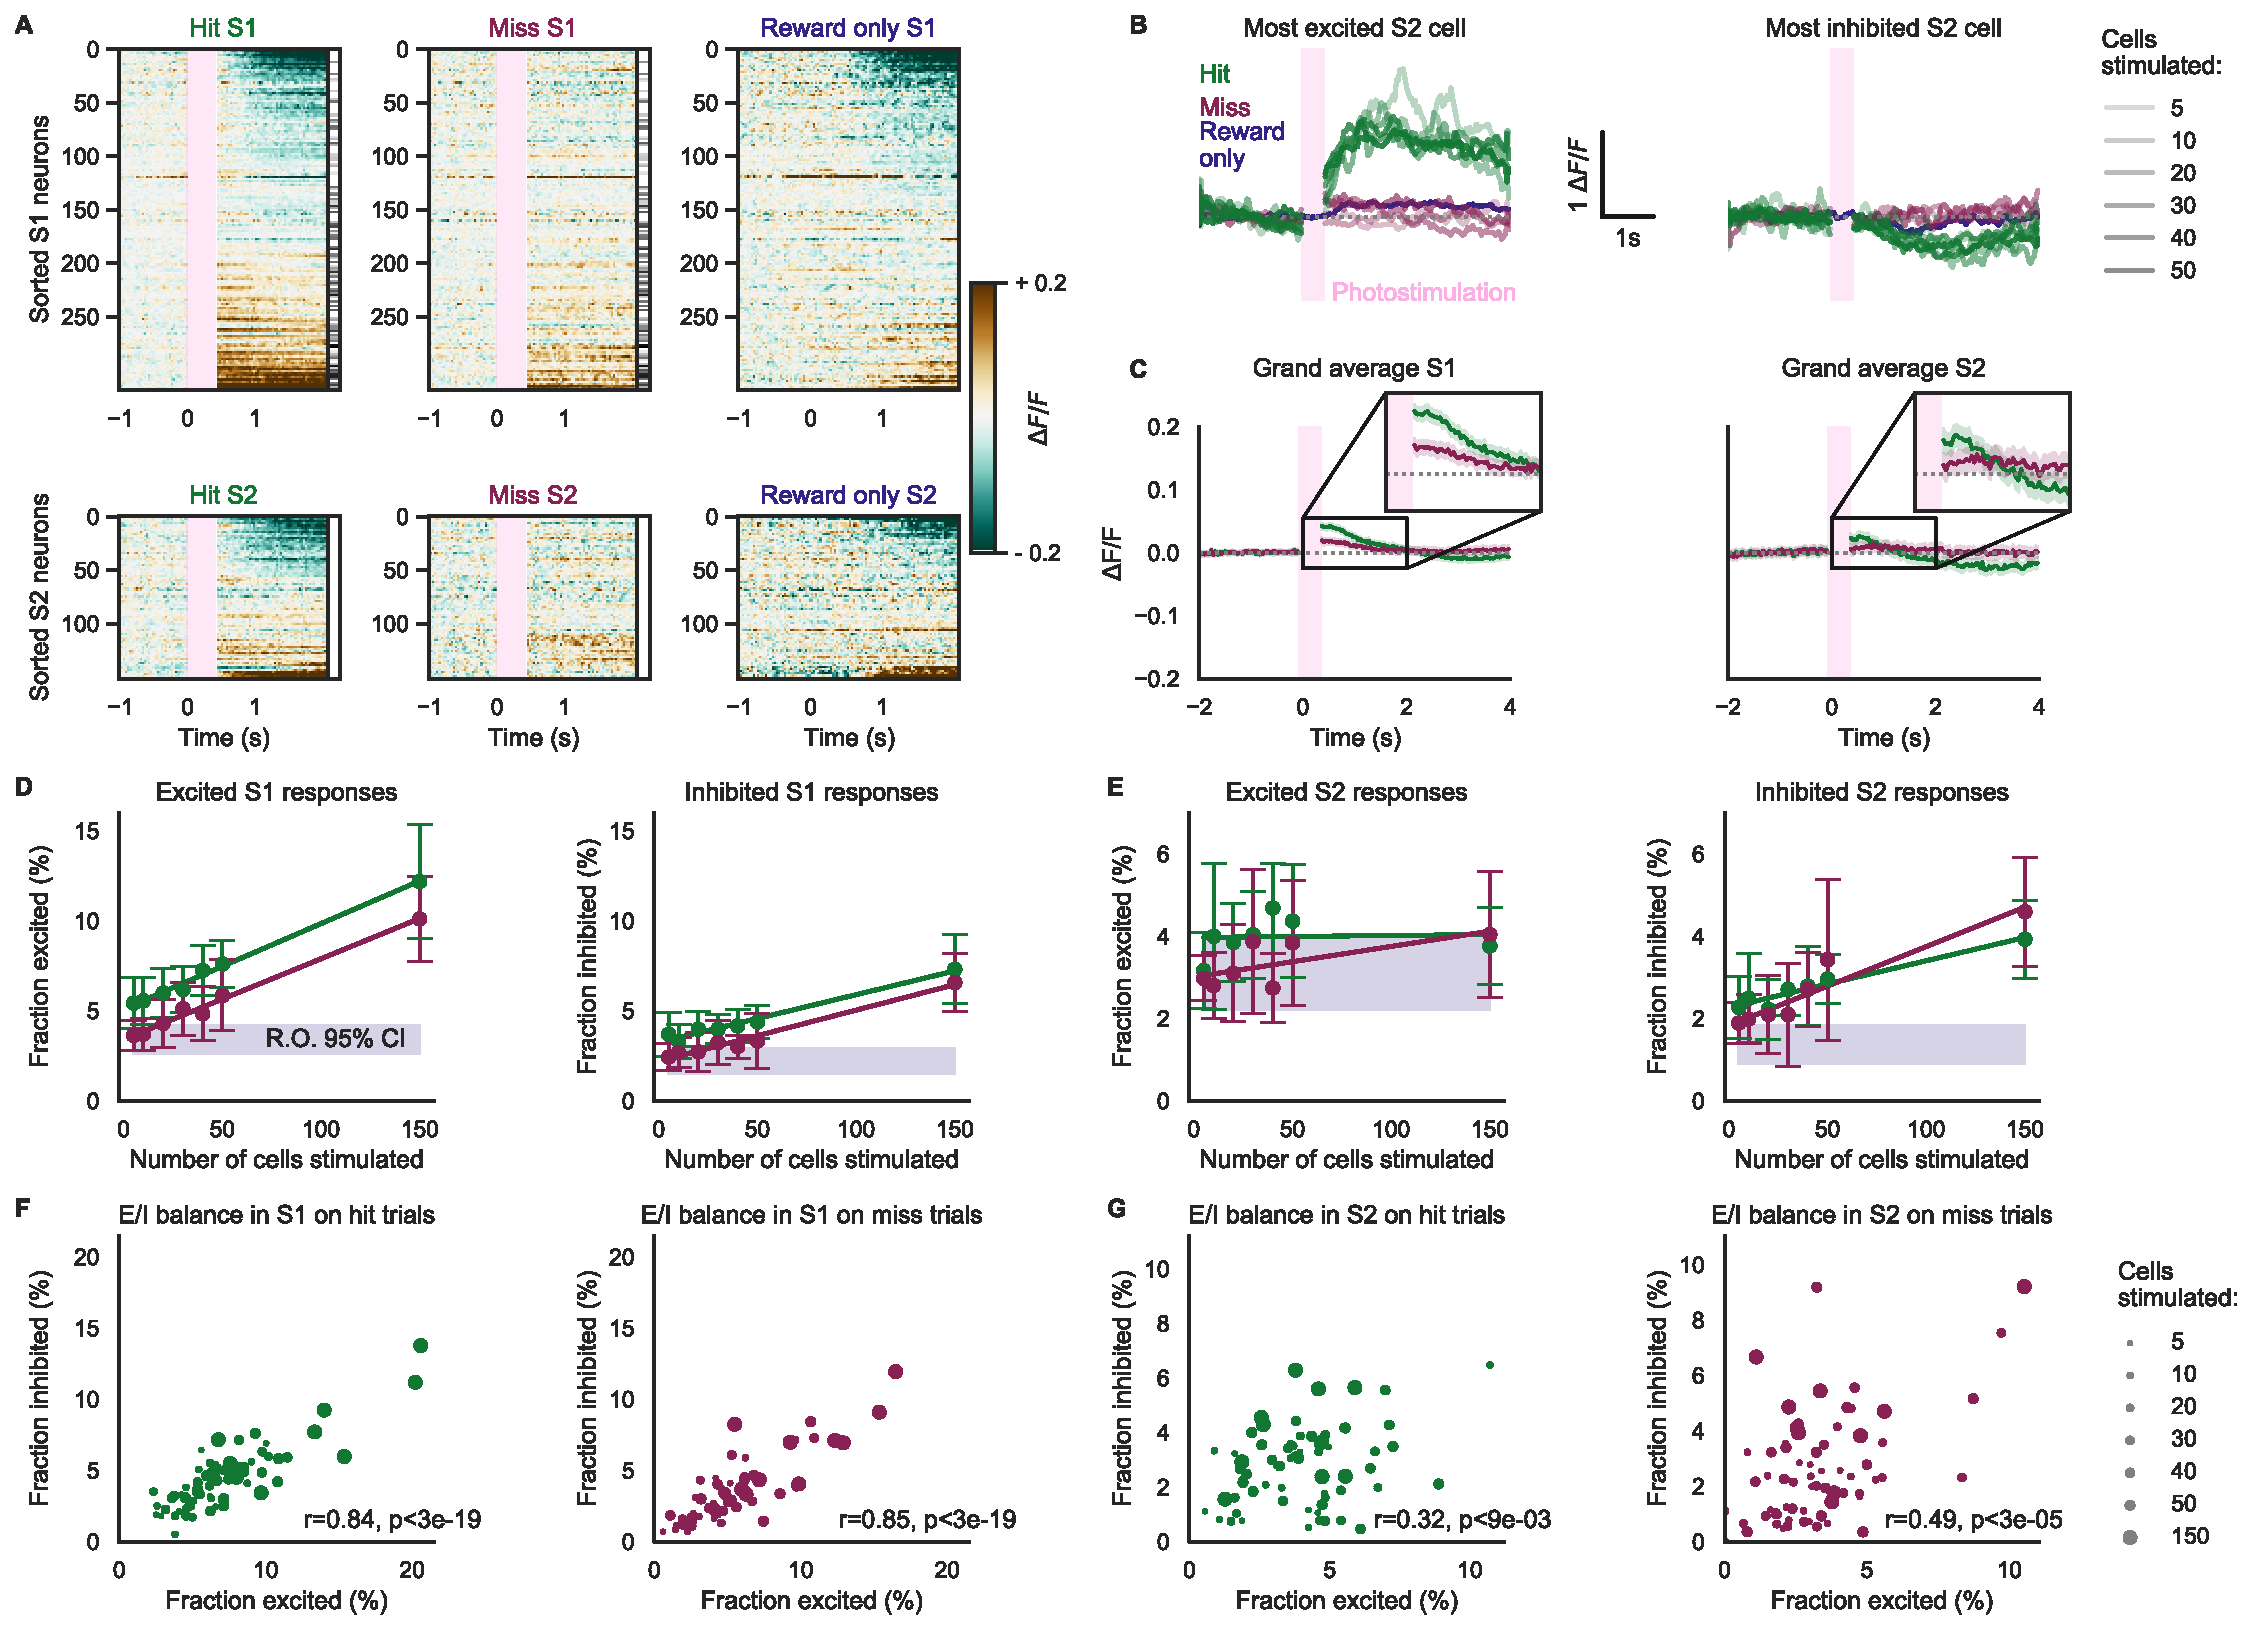
\includegraphics[scale=0.45]{figures/basic-analysis.pdf}
\caption[\textbf{name}]{
\textbf{name}. \textbf{(A)} Raster plots showing the trial averaged response to trial types (Left: hit, Middle: miss, Right: reward only) to photostimulation (pink vertical bar, hit/miss)  and/or reward (hit/reward only) of individual cells from a single session. Data were baselined to the pre-stimulus mean on a cell-wise basis before averaging. Cells are sorted by the pairwise correlation between their trial averaged responses across all three trial types (methods). A clear excitatory and inhibitory response is elicited in S1 and S2 on hit trials that cannot be solely attributed to reward. The intensity of the bar on the right hand side of the hit and miss rasters is proportional to the number of times each cell was directly targeted by the photostimulation beam. Trials in which 150 cells were stimulated were removed for display. Data are blanked while the photostimulation laser was on (pink bar). \textbf{(B)} \textit{Left}: Example S2 cell excited on hit trials (green) but showing no response to miss trials (red) or reward only trials (blue). Each line shows an individual trial. The transparency of the line indicates the number of cells stimulated in S1. Individual trials were baslined to the pre-stimulus mean. Right: Example S2 cell inhibited on hit trials. Trials in which 150 cells were stimulated were removed for display. \textbf{(C)} Average population response to hit and miss trials across all sessions. Traces are averaged across cells, trials and sessions for a given trial type. Individual trials were baselined to the pre-stimulus mean. Trials in which 150 cells were stimulated were removed for display. \textbf{(D)} Function mapping the response in S1 on hit and miss trials to the number of cells stimulated in S1. Left: The fraction of excited cells in S1 maps linearly to the number of cells photostimulated on both hit and miss trials. Right: The fraction of inhibited cells in S1 maps linearly to the number of cells photostimulated on both hit and miss trials. The shaded purple bar shows the fraction of excited or inhibited cells in S1 on reward only (R.O.) trials. \textbf{(E)} Function mapping the response in S2 on hit and miss trials to the number of cells stimulated in S1. Left: There is no relationship between the fraction of excited cells in S2 and the number of cells stimulated in S1 on hit trials or miss trials. The shaded purple bar shows the fraction of excited or inhibited cells in S2 on reward only trials. Right: The fraction of inhibited cells in S2 maps linearly to the number of cells photostimulated in S1 on both hit and miss trials. \textbf{(F)} Population E/I balance in S1 following photostimulation. The fraction of cells excited by photostimulation in S1 is highly correlated with the fraction of cells inhibited both on hit trials (left) and miss trials (right). The size of the circle indicates the number of cells photostimulated. \textbf{(G)} Population E/I balance in S2 following photostimulation in S1. The fraction of cells excited by photostimulation in S1 is significantly correlated with the fraction of cells inhibited both on hit trials (left) and miss trials (right). However the magnitude of the correlation is lower than in S1. The size of the circle indicates the number of cells photostimulated. 

} 
\label{fig:basic-analysis}
\end{figure}

fjkdlsflksdj





\section{Logistic regression classification of trial type}



\section{Stimulus signal-to-noise ratio}

